% Article template for Mathematics Magazine
% Revised 7/2002  Thanks for Greg St. George
\documentclass[12pt]{article}
\usepackage{amssymb}
\usepackage[ngerman]{babel}
\usepackage[utf8]{inputenc}
\usepackage{amsmath}
\usepackage{amsthm}
\renewcommand{\baselinestretch}{1.2}
%This is the command that spaces the manuscript for easy reading
\newtheorem{zeige}{Zeige}


%todo 
\usepackage[colorinlistoftodos,prependcaption,textsize=tiny]{todonotes}
\usepackage{xargs}                      % Use more than one optional parameter in a new commands
\newcommandx{\QUESTION}[2][1=]{\todo[linecolor=none,backgroundcolor=blue!15,bordercolor=none,#1]{\textbf{QUESTION: }#2}}



\begin{document}
%\thispagestyle{empty}
\begin{center}
\Large
% TITLE GOES HERE
Logik und Komplexität  \textsc{ Übung 7 }
\end{center}

\begin{flushright}
Denis Erfurt, 532437\\
HU Berlin \\

\vspace{2 mm}

\end{flushright}

\subsubsection*{Aufgabe 1)}
\begin{zeige}
  C ist Hanf-lokal in S $\Rightarrow $ C ist FO-definierbar in S
\begin{proof}
  % Es genügt die kontrapositon zu zeigen:\\
  % C ist nicht FO-definierbar in S $\Rightarrow $ C ist nicht Hanf-lokal in S \\
  
  Es exestiert eine Zahl $r\in\mathbb{N}$, so dass für alle $\mathfrak{A},\mathfrak{B}\in S$ gilt: 
  \[ \text{Falls } \mathfrak{A} \rightleftarrows_r \mathfrak{B} \text{, so } (\mathfrak{A}\in C \Leftrightarrow \mathfrak{B}\in C ) \] 

  $\Rightarrow $ für jeden r-Umgebungstyp $\varrho$ gilt:
  \begin{center}
    Falls $\#_\varrho(\mathfrak{A}) = \#_\varrho (\mathfrak{B})$, so $(\mathfrak{A}\in C \Leftrightarrow \mathfrak{B}\in C )$\\
  \end{center}
  
  % Sei $r=3^m$ sowie $\phi\in FO[\sigma]$ mit $qr(\phi) = m$:

  % $\Rightarrow$
  
  % Sei r=$3^m$: für jeden $3^m$-Umgebungstyp $\varrho$ gilt: $\#_\varrho(\mathfrak{A}) = \#_\varrho (\mathfrak{B})$\\
  
  Da es sich bei S um endliche Strukturen handelt sind $\mathfrak{A}$ und $\mathfrak{B}$ ebenfalls endlich. Sei $r=3^m$.
  \QUESTION[inline]{Kann ich $k=0$ so annähmen, oder muss ich das für alle $k$ berücksichtigen?}
  O.b.d.A. ist $k=0$. Somit sind alle Bedingungen vom Satz von Hanf erfüllt. Somit gilt 
  \begin{center}
    Falls $\mathfrak{A} \approx_m \mathfrak{B}$, so $(\mathfrak{A}\in C \Leftrightarrow \mathfrak{B}\in C )$
  \end{center}
  
  Somit gibt es nach Ehrenfeucht eine (FO) Hintikka Formel, die die Gewinnstrategie für Dup. auf m Runden EF Spiel für $\mathfrak{A}$ und $\mathfrak{B}$ beschreibt.
  

  \begin{center}
    Falls $\mathfrak{B} \models \phi^m_{A}$, so $(\mathfrak{A}\in C \Leftrightarrow \mathfrak{B}\in C )$
  \end{center}

  Sei $Q\subseteq m-Typen_0[\sigma]$ so dass f.a. $\mathfrak{A},\mathfrak{B}\in C$ gilt: $\mathfrak{B} \models \phi^m_{A} \Rightarrow \phi^m_{A}\in Q$
  
  \[ \psi := \bigvee_{\phi \in Q} \phi \] 
  Da $Q$ endlich ist exestiert ein solches $\psi\in FO[\sigma]$.
  Somit gilt 
  $$ \mathfrak{A}\in C \Rightarrow \mathfrak{A} \models \psi $$
  Somit ist $C:=\{\mathfrak{A}\in S: \mathfrak{A}\models \psi\}$ und damit FO-definierbar in S.

  
  
  
\end{proof}
\end{zeige}

\subsubsection*{Aufgabe 2)}
Idee: Zerteilung mit dem Kompositionslemma.

\QUESTION[inline]{konstanten überführen in relationen}
Sei $\mathcal{A}_f := \left. \mathcal{A} \right|_{M_f^{\mathcal{A}}}$.

$\Rightarrow \mathcal{A} := \bigsqcup_{ f\subseteq \sigma_{k, l } } \mathcal{A}_f$

Nach dem Kompositionslemma folgt: \\

Falls für alle $\mathcal{A}_f,\mathcal{B}_f$ gilt $\mathcal{A}_f \approx_m \mathcal{B}_f \Rightarrow \mathcal{A} \approx_m \mathcal{B}$

Beobachtung 1: für alle $P\in\sigma_{k, l}: P^{\mathcal{A}_f}=
\begin{cases}
 A^{\mathcal{A}_f}&P\in f\\
 \{\}&P\notin f
\end{cases}$

Beobachtung 2: Für alle $f\subseteq \sigma_{k, l}$ hängt die Gewinnstrategie von Dup. im $EF(\mathcal{A}_f,\mathcal{B}_f)$-Spiel \textbf{nur} von den Universen $A^{ \mathcal{A}_f },B^{ \mathcal{B}_f }$ ab.

$\Rightarrow$ um zu zeigen $\mathcal{A}_f \approx_m \mathcal{B}_f$ genügt es demnach zu Zeigen: $\mathcal{A}'_f \approx_m \mathcal{B}'_f$. Dabei sind $\mathcal{A}'_f,\mathcal{B}'_f$ $\sigma={}$-Strukturen mit $A^{ \mathcal{A}'_f } = A^{ \mathcal{A}_f }$ sowie $B^{ \mathcal{B}'_f } = B^{ \mathcal{B}_f }$.

Falls $|A^{ \mathcal{A}'_f }|=|B^{ \mathcal{B}'_f }|$: dann sind beide Strukturen isomorph und somit gilt: $\mathcal{A}'_f \approx_m \mathcal{B}'_f$.

Falls $|A^{ \mathcal{A}'_f }|,|B^{ \mathcal{B}'_f }| > 2^m$:

\QUESTION[inline]{Was muss bei einer Menge übereinstimmen? Falls Sp. eine Menge auswählt. was kann Dup als valide menge auswählen? müssen sie Gleiche Kardinalität besitzen}








\subsubsection*{Aufgabe 3. a)}
\begin{zeige}
  $2-COL$ ist nicht Fo-definierbar in $DGraph$\\
  $\Rightarrow$ Für jedes $r\in\mathbb{N}$ exestiert ein $\mathfrak{A}_r \in  2-COL$ und $\mathfrak{B}_r \in DGraph \setminus 2-COL$ mit $\mathfrak{B}_r\rightleftarrows_r \mathfrak{A}_r$ :\\
  
  \begin{proof}
    
    Sei $\mathfrak{A}_r$ eine Struktur bestehend aus 2 gerichteten Kreisen mit je 2r+3 Knoten.
    Sei $\mathfrak{B}_r$ ein Großer Kreis mit $4r+6$ Knoten.

    Für alle $a\in A$ sieht der r-Umgebungstyp $\mathfrak{N}_r^{\mathfrak{A}_r}(a)$ wie eine Linie aus mit $2r+1$ Knoten.\\
    Auch gilt für alle $a\in A, b\in B$: 
    $$(\mathcal{N}_r^{\mathfrak{A}_r}(a),a) \cong (\mathcal{N}_r^{\mathfrak{B}_r}(b),b)$$
    Somit gilt für jeden r-Umgebungstyp $\varrho: \#_\varrho(\mathfrak{A}_r)=\#_\varrho(\mathfrak{B}_r)$ und somit: $$\mathfrak{A}\rightleftarrows_r \mathfrak{B}_r$$
    
    Klar ist auch: $\mathfrak{A}_r\in DGraph\setminus 2-COL$, da die Kreise jeweils eine ungerade Anzahl an Knoten besitzen. Jedoch ist $\mathfrak{B}_r\in 2-COL$.\\
    $\Rightarrow $Somit ist $2-COL$ nicht FO-definierbar in $DGraph$.
  \end{proof}
\end{zeige}
\subsubsection*{Aufgabe 3. b)}
\begin{zeige}
  $3-COL$ ist nicht FO-definierbar in DGraph.
  $\Rightarrow $
  Für jedes $r\in\mathbb{N}$ exestiert ein $\mathfrak{A}_r \in  3-COL$ und $\mathfrak{B}_r \in DGraph \setminus 3-COL$ mit $\mathfrak{B}_r\rightleftarrows_r \mathfrak{A}_r$ :\\
  \begin{proof}
    Sei $\mathcal{K}_r$ ein Graph mit: $V=\{1,...,r\}$ sowie $
    E=
    \{(n,n+1): n\in\{1,...,r-1\}\} \cup 
    \{(n,n+2): n\in\{1,...,r-2\}\} \cup
    \{(n-1,1),(n,1),(n,2)\}$
    
    \begin{center}
      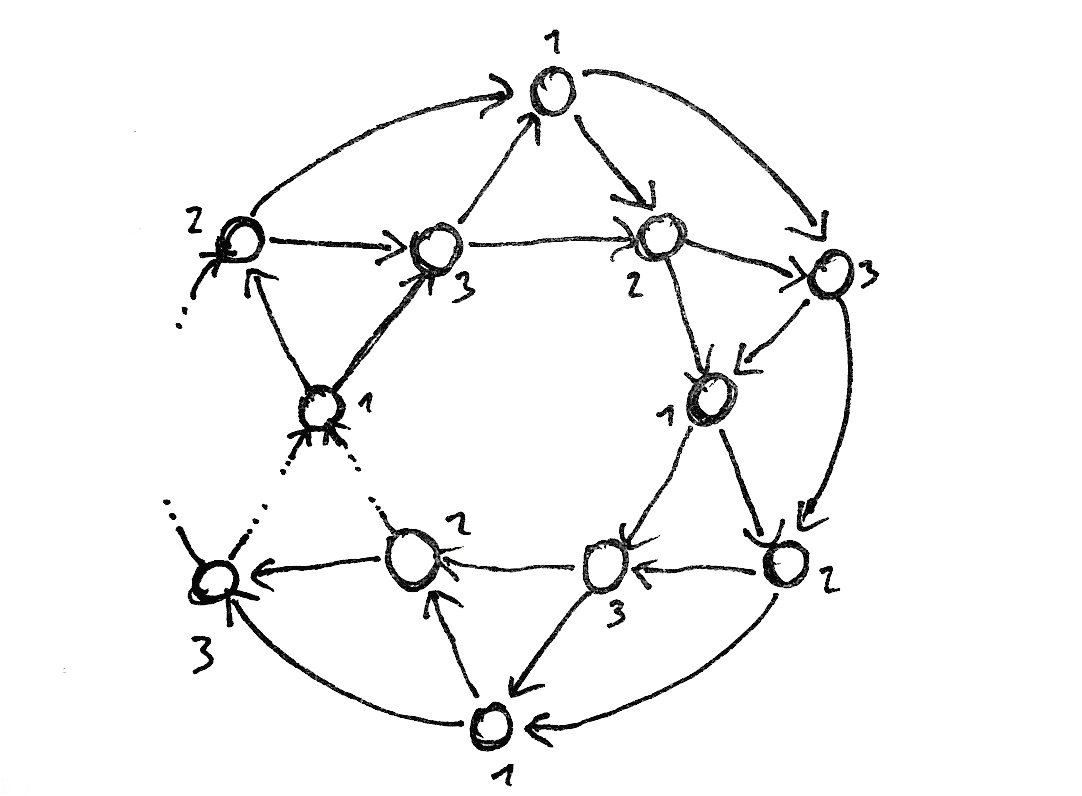
\includegraphics[scale=0.2]{circle.jpg}
    \end{center}
    
    $\mathcal{K}_r \in 3-COL \Leftrightarrow r=6n$ für $n\in\mathbb{N}^+$
    
    Für ein Kreis $\mathcal{K}_{r+1}$ und ein Beliebigen $a\in V$ sieht die r-Umgebung $\mathcal{N}^{\mathcal{K}_{r+1}}(a)$ folgendermaßen aus:
    
    \begin{center}
      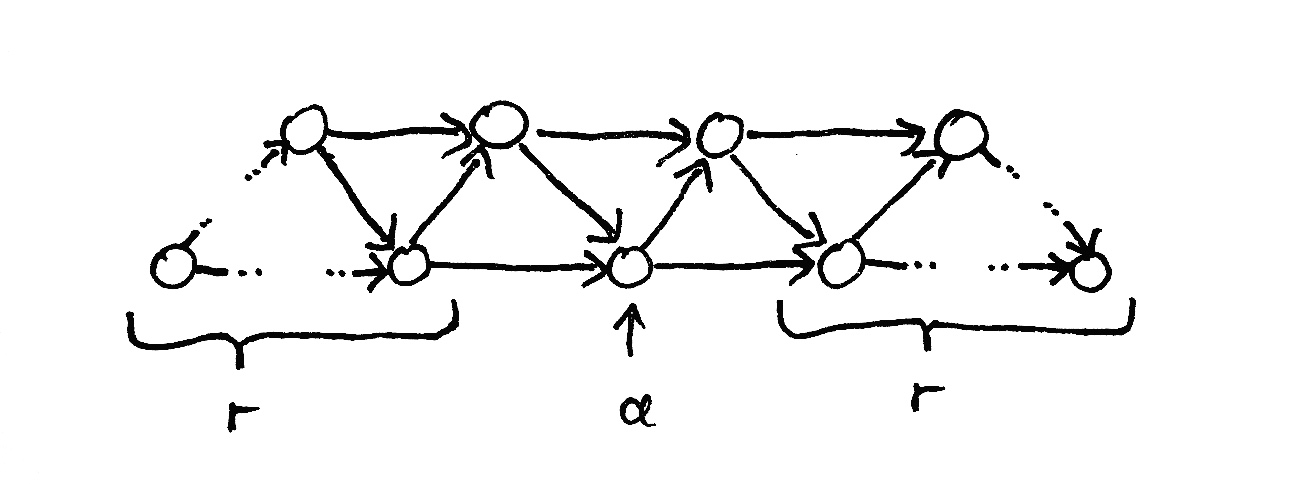
\includegraphics[scale=0.2]{r-env.jpg}
    \end{center}
    
    Außerdem gilt für $a\in \mathcal{K}_p,b\in \mathcal{K}_q$ mit $p,q\geq r+1$: 
    $$(\mathcal{N}_r^{\mathcal{K}_p}(a),a) \cong (\mathcal{N}_r^{\mathcal{K}_q}(b),b)$$
    
    
    Sei $\mathfrak{A}_r := \mathcal{K}_{6r+6}\cup \mathcal{K}_{6r+8} \cup \mathcal{K}_{6r+10}$
    
    $\Rightarrow $ f.a. $r\in \mathbb{N}$: $\mathfrak{B}_r\in DGraph\setminus 3-COL$
    
    Sei $\mathfrak{B}_r := \mathcal{K}_{18r+24}$
    
    $\Rightarrow $ f.a. $r\in \mathbb{N}$: $\mathfrak{B}_r\in 3-COL$
    
    Da $|A| = |B| \Rightarrow $ für jeden r-Umgebungstyp $\varrho$: $ \#_\varrho(\mathfrak{A}_r)=\#_\varrho(\mathfrak{B}_r) $
    
    und somit $\mathfrak{B}_r\rightleftarrows_r \mathfrak{A}_r$
    
  \end{proof}
\end{zeige}
\subsubsection*{Aufgabe 4)}

\end{document}
